Vyhodnocení je rozděleno na dvě části -- a~to sice na první, která se zabývá kvalitativním vyhodnocením detektoru (tedy jak kvalitní detekce systém provádí) a~druhou, která udává celkovou úspěšnost systému (kolik z testovaných značek dokáže systém správně detekovat a s jakou chybovostí systém pracuje).

%%%%%%%%%%%%%%%%%%%%%%%%%%%%%%%%%%%%%%%%%%%%%%%%%%%%%%%%%%%%%%%%%%%%%%%%%%%%%%%%%%%%%%%%%%%

\section{Kvalitativní vyhodnocení}
Pokud je značka dobře viditelná a~bez znatelného poškození, model ji ve většině případů správně detekuje s~90-100$\,\%$ jistotou. Problém modelu dělají značky malé, pod velkým úhlem, poničené či vybledlé, a~také občasná záměna pozadí za objekt (pokud má objekt podobný tvar a~barvu), jak lze vidět na obrázcích \ref{fig:multipleDetections}, \ref{fig:wrongClassDetections}, \ref{fig:missingDetections} a \ref{fig:backgroundDetections}. Selhání potlačení nemaximálních hodnot, tzn. některá ze značek je detekována vícekrát, je nejméně často se vyskytující chybou.

\begin{figure}[H]
    \centering
    \tmpframe{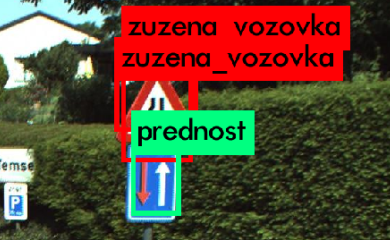
\includegraphics[width=0.495\linewidth]{figures/vyhodnoceni/multiple_detection_1.png}}\hfill
    \tmpframe{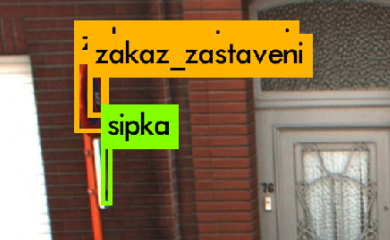
\includegraphics[width=0.495\linewidth]{figures/vyhodnoceni/multiple_detection_2.png}}
    \caption{Značky jsou správně detekovány i klasifikovány, ovšem některé více-násobně. To značí selhání potlačení ne-maximálních hodnot.}
    \label{fig:multipleDetections}
\end{figure}

\begin{figure}[H]
    \centering
    \tmpframe{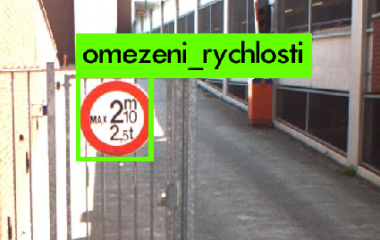
\includegraphics[width=0.495\linewidth]{figures/vyhodnoceni/wrong_class_1.png}}\hfill
    \tmpframe{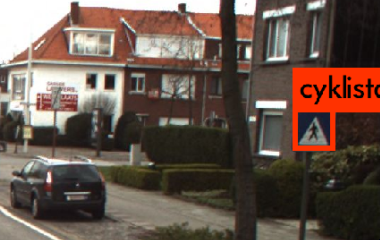
\includegraphics[width=0.495\linewidth]{figures/vyhodnoceni/wrong_class_2.png}}
    \caption{Nesprávně klasifikované dopravní značky.}
    \label{fig:wrongClassDetections}
\end{figure}

\begin{figure}[H]
    \centering
    \tmpframe{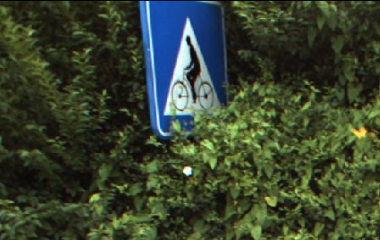
\includegraphics[width=0.495\linewidth]{figures/vyhodnoceni/missing_detection_1.png}}\hfill
    \tmpframe{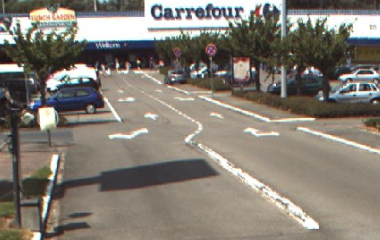
\includegraphics[width=0.495\linewidth]{figures/vyhodnoceni/missing_detection_2.png}}
    \caption{Značky, které nebyly detekovány.}
    \label{fig:missingDetections}
\end{figure}

\begin{figure}[H]
    \centering
    \tmpframe{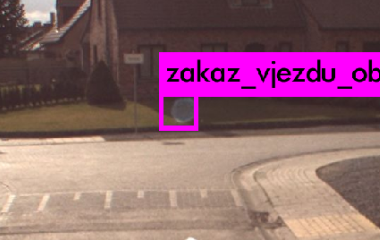
\includegraphics[width=0.495\linewidth]{figures/vyhodnoceni/background_detection_1.png}}\hfill
    \tmpframe{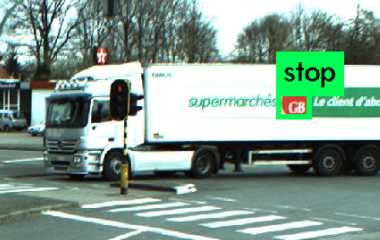
\includegraphics[width=0.495\linewidth]{figures/vyhodnoceni/background_detection_2.png}}
    \caption{Záměna pozadí za detekované objekty.}
    \label{fig:backgroundDetections}
\end{figure}

 I~přes to, že má YOLO problémy s~dokonalou lokalizací objektů, predikované boxy v mnoha případech ohraničují celou značku a~to poměrně přesně. Příklad několika správných detekcí za zhoršených podmínek lze vidět na obrázcích \ref{fig:correctDetectionsLuminescence}, \ref{fig:correctDetectionsObstacle}, \ref{fig:correctDetectionsSmall} a \ref{fig:correctDetectionsBroken}.
 
\begin{figure}[H]
    \centering
    \tmpframe{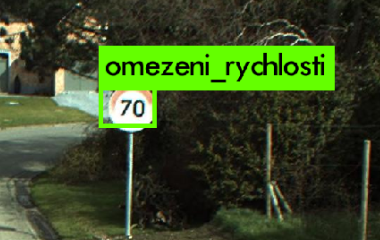
\includegraphics[width=0.495\linewidth]{figures/vyhodnoceni/correct_luminescence_1.png}}\hfill
    \tmpframe{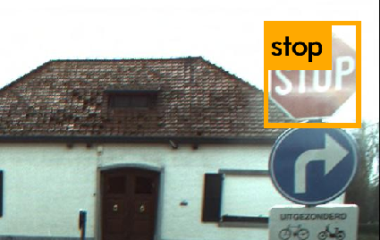
\includegraphics[width=0.495\linewidth]{figures/vyhodnoceni/correct_luminescence_2.png}}
    \caption{Správné detekce i za zhoršených světelných podmínek.}
    \label{fig:correctDetectionsLuminescence}
\end{figure}

\begin{figure}[H]
    \centering
    \tmpframe{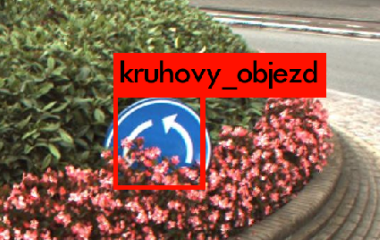
\includegraphics[width=0.495\linewidth]{figures/vyhodnoceni/correct_obstalce_1.png}}\hfill
    \tmpframe{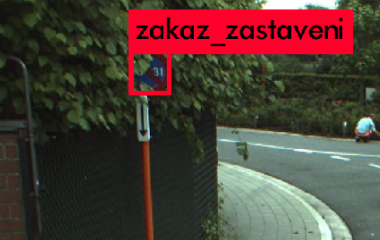
\includegraphics[width=0.495\linewidth]{figures/vyhodnoceni/correct_obstalce_2.png}}
    \caption{Správné detekce i při částečném překrytí.}
    \label{fig:correctDetectionsObstacle}
\end{figure}

\begin{figure}[H]
    \centering
    \tmpframe{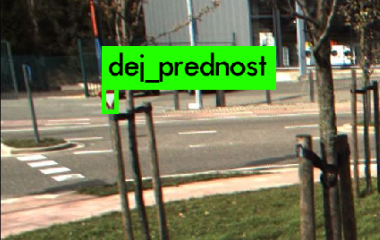
\includegraphics[width=0.495\linewidth]{figures/vyhodnoceni/correct_small_1.png}}\hfill
    \tmpframe{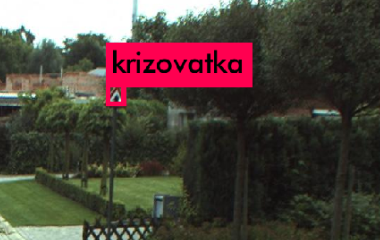
\includegraphics[width=0.495\linewidth]{figures/vyhodnoceni/correct_small_2.png}}
    \caption{Správné detekce i přes velmi malou velikost dopravních značek.}
    \label{fig:correctDetectionsSmall}
\end{figure}

\begin{figure}[H]
    \centering
    \tmpframe{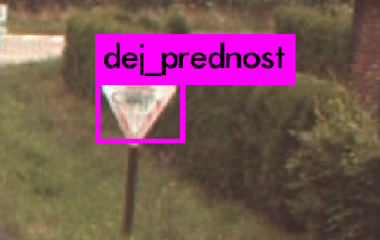
\includegraphics[width=0.495\linewidth]{figures/vyhodnoceni/correct_broken_1.png}}\hfill
    \tmpframe{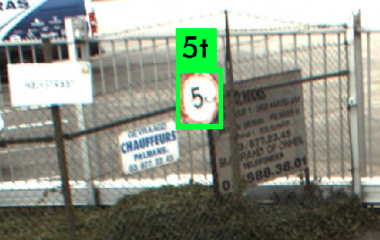
\includegraphics[width=0.495\linewidth]{figures/vyhodnoceni/correct_broken_2.png}}
    \caption{Správné detekce i přes nízkou kvalitu či poškození dopravních značek.}
    \label{fig:correctDetectionsBroken}
\end{figure}

%%%%%%%%%%%%%%%%%%%%%%%%%%%%%%%%%%%%%%%%%%%%%%%%%%%%%%%%%%%%%%%%%%%%%%%%%%%%%%%%%%%%%%%%%%%

\section{Kvantitativní vyhodnocení}
Ke kvantitativnímu vyhodnocení úspěšnosti byl využit zejména repozitář mAP\footnotemark, který byl v~rámci této práce doplněn o~vykreslení ROC (\emph{Receiver operating characteristic}) křivky a~analýzu chyb.

\footnotetext{\url{https://github.com/Cartucho/mAP}}

\subsection*{Výsledky při použití reálné datové sady}
\label{vysledkyRealDataset}
Při použití reálné datové sady pro trénování je možné postupovat tak, že se datová sada rozdělí na dvě části. První část jsou data, na kterých bude detektor/klasifikátor trénován a~skládá se z~trénovací a~validační sady. Druhou částí jsou pak data, na kterých se vyhodnotí úspěšnost natrénovaného modelu a~tato data jsou běžně označována jako testovací. Pro vyhodnocení není potřeba tolik dat, jako pro trénování a~validaci, proto byla tato část menší, a~to přesně v~poměru 2:1. Belgická datová sada se skládá z~cca. 9000 snímků (nepočítaje negativní datovou sadu), takže pro trénování bylo využíváno $\sim6000$ a~pro testování $\sim3000$ snímků. Dosažené výsledky se pohybovaly kolem $\sim60\,\%$ mAP, což je téměř dvakrát více, než se podařilo dosáhnout v~práci \cite{tsdYolo} používající YOLO první verze. K~nárůstu úspěšnosti přispěla zejména modifikace třetí verze YOLO, razantně zlepšující detekci malých objektů.


\subsection*{Výsledky při použití syntetické datové sady}
\label{vysledkySyntDataset}
Při trénování na syntetických datech bylo možné využít veškeré snímky z~Belgické datové sady k~testování. Jako nejoptimálnější počet generovaných dat podle tabulky \ref{tab:pocetSnimkuUspesnost} vyplývá $1000$ snímků na třídu. Výsledky se pohybovaly kolem $\sim80\,\%$ mAP. Lepší úspěšnosti dosahoval způsob generování s~transparentními značkami (o~několik bodů mAP lepší oproti generování s~ořezanými značkami). Zlepšení o~dva body mAP bylo dosaženo pomocí přimíchání malého množství reálných snímků do syntetické datové sady.

\subsection*{Porovnání výsledků}
Porovnání výsledků modelů trénovaných na reálných a~syntetických datech při použití různých velikostí vstupní vrstvy lze vidět na obrázku \ref{fig:porovnaniMapMs}.

\begin{figure}[H]\centering
    \centering
    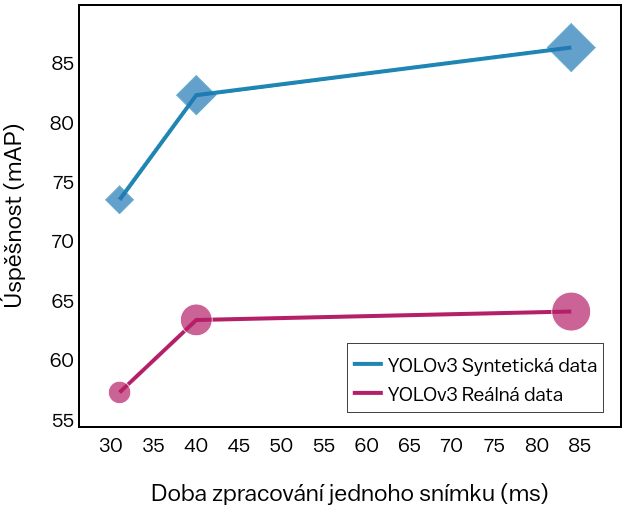
\includegraphics[width=0.6\linewidth]{figures/vyhodnoceni/map_ms_tradeoff.png}
    \caption{Porovnání závislosti úspěšnosti na době zpracování jednoho snímku třech modelů (zleva) YOLOv3-320, YOLOv3-416 a~YOLOv3-608 trénovaných na syntetických a~reálných datech. Zvětšující se velikost bodů reprezentuje velikosti vstupní vrstvy modelů. Z~grafu lze vidět, že čím větší vstupní vrstva se použije, tím lepších výsledků detekce je dosaženo, ale také se tím prodlouží doba detekce. Za nejvhodnější lze tedy považovat prostřední model YOLOv3-416, který poskytuje nejlepší kompromis (tzv. \emph{tradeoff}) mezi úspěšností a~časem. Výsledky byly získány na GeForce 840M.}
    \label{fig:porovnaniMapMs}
\end{figure}


\section{Analýza chyb}
Výsledné modely měly poměrně vysoký počet falešně pozitivních predikcí, proto bylo vhodné zjistit, co dělá systému problém. Poté bylo možné navrhnout řešení a~dosahovat tak lepších výsledků. Použita byla metodika analýzy chyb popsaná v~práci~\cite{errorAnalysis}. Predikce je buď to správná, nebo je zařazena do jedné z~následujících tříd~\cite{yolov1}.

\begin{itemize}
    \item \textbf{Správná predikce} -- správná třída, IoU $> 0.5$.
    \item \textbf{Chyba lokalizace} -- správná třída, $\text{IoU} \in \interval({0.1,0.5})$.
    \item \textbf{Podobné} -- podobná třída, $\text{IoU} > 0.1$.
    \item \textbf{Ostatní} -- nesprávná třída, $\text{IoU} > 0.1$.
    \item \textbf{Detekce pozadí} -- jakákoli detekce s~$\text{IoU} < 0.1$.
\end{itemize}

Více-násobná detekce jednoho objektu se dá také považovat za chybu (selhání potlačení nemaximálních hodnot), a~proto bylo vyhodnocení doplněno o~třídu vícenásobné detekce. Naopak kvůli nedostatku času nejsou detekce nesprávných tříd rozděleny do kategorií \emph{podobné} a~\emph{ostatní}. Vizualizovanou distribuci chyb obou modelů lze vidět na obrázku \ref{fig:analyzaChyb}.

\begin{figure}[H]\centering
    \centering
    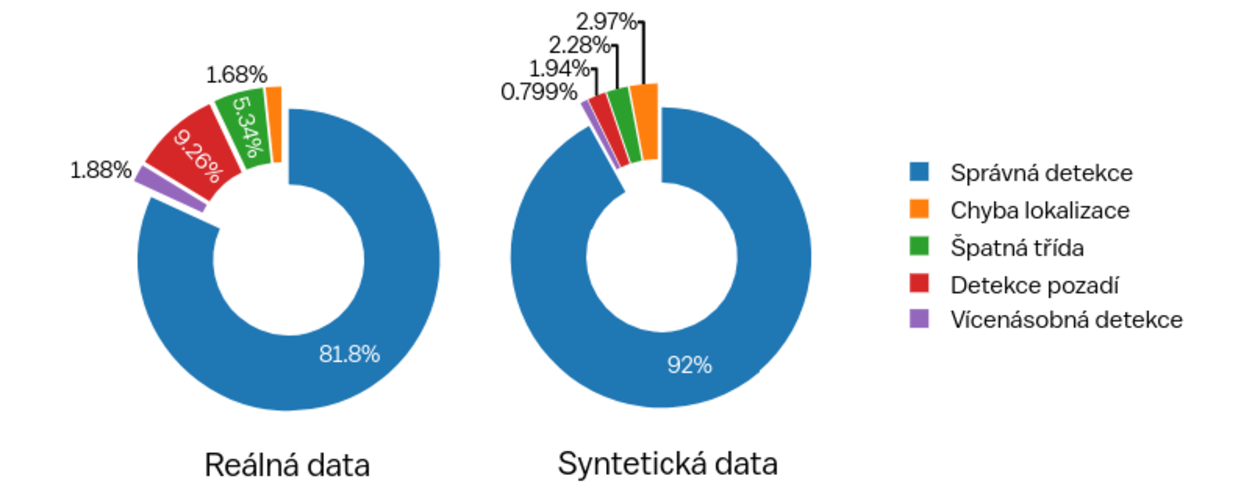
\includegraphics[width=0.99\linewidth]{figures/vyhodnoceni/error_analysis.pdf}
    \caption{Analýza chyb dvou modelů, trénovaných na reálných a~syntetických datech. Model trénovaný na reálných datech (\textbf{vlevo}) má větší problém se záměnou pozadí s~objekty a~také nesprávné určování tříd značek. To je zapříčiněno nedostatečným množstvím informací o~některých třídách (malou velikostí datové sady). Naopak má nižší chybovost lokalizace, což znamená že dokáže predikované boxy lépe zarovnat na detekovanou značku. Pokles v~úspěšnosti mAP zapříčiňují také falešně negativní vzorky, které do grafu nejsou zahrnuty.}
    \label{fig:analyzaChyb}
\end{figure}